\documentclass[12pt]{article}
\usepackage[margin=1in]{geometry}
\usepackage{amsmath}
\usepackage{amssymb}
\usepackage{amsthm}
\usepackage{physics}
\usepackage{graphics}

\theoremstyle{plain}
\newtheorem{theorem}{Theorem}
\newtheorem{corollary}{Corollary}
\newtheorem{proposition}{Proposition}

\theoremstyle{definition}
\newtheorem{definition}{Definition}
\newtheorem{question}{Question}
\newtheorem{example}{Example}

\newcommand{\ve}{\varepsilon}
\newcommand{\Real}{\mathbb{R}}
\newcommand{\CD}[1]{\mathcal{C}^{#1}}

\title{Multivariable Calculus}
\author{Jonathan Lin}
\date{\today}

\begin{document}
\maketitle

\section{Two Important Theorems}

In this section we discuss the \textit{Implicit Function Theorem} and the \textit{Inverse Function Theorem}, the two most important results in differential calculus. In their essence they are about solving certain systems of equations and determining the dependent and independent variables in a system.

\subsection{Inverse Function Theorem Motivation}
The main idea of the inverse function theorem is that given a suitably ``nice'' mapping, one might be able to determine whether or not an inverse mapping exists and it might possibly have some nice properties. To motivate the statements that our theorems have we will explore some examples in the one dimensional case. First, we might recall that if $f'(x) > 0$ on some interval $[a, b]$ this implies that $f$ is increasing on $[a, b]$. Let's consider a related question: Suppose we know at some point $x$ that $f'(x) = 0$. Does that mean there is some interval containing $x$ where $f$ is increasing? The answer is no. To see this, we might consider the graph of the function $f(x) = x^2\sin(1/x)$:

\begin{figure}[h]
	\centering
	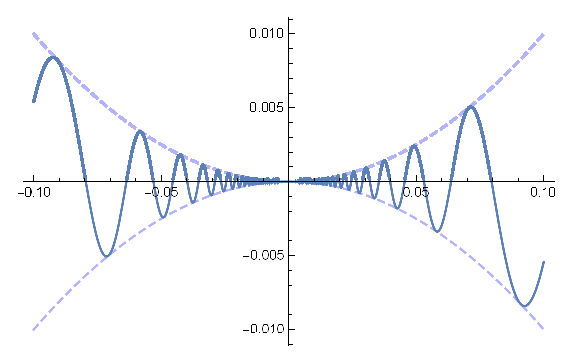
\includegraphics{plots_gr1.eps}
	\caption{The graph of $f(x) = x^2\sin(1/x)$}
	\label{fig:plots_gr1}
\end{figure}

It is straightforward to see that $f$ is differentiable everywhere but $0$, and if we further define $f$ so that $f(0) = 0$, we see that $f(x)$ is differentiable at $0$ with $f'(0) = 0$.

Similarly, we can consider the function 
\[f(x) = \begin{cases} 0 & x = 0 \\ \frac{x}{2} + x^2\sin(1/x) & \text{otherwise.} \end{cases}\]
Then $f'(0) = 1/2$. However, it is straightforward to show that $f(x)$ is not increasing on any interval containing $f(0) = 0$. That is, there are points as close to $0$ as we would like where the derivative is less than $0$.

\begin{figure}[h]
	\centering
	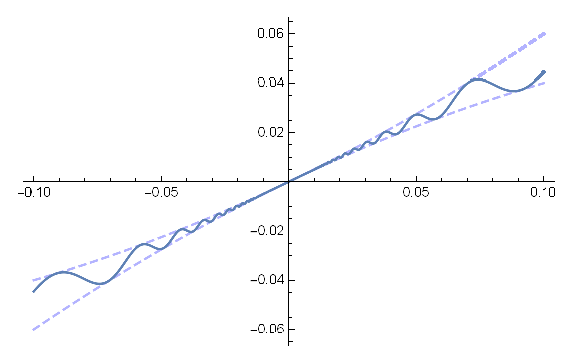
\includegraphics{plots_gr2.eps}
	\caption{The graph of $f(x) = \frac{x}{2} + x^2\sin(1/x)$}
	\label{fig:plots_gr2}
\end{figure}

So simply the derivative being non-zero at a point does not give us an interval containing that point where the function $f$ is increasing. In particular, there is no interval around that point where $f$ is \textit{invertible} when restricted to that interval. So what went wrong here? Let's take the derivative of $x^2\sin(1/x)$ when $x \neq 0$:
\[\frac{d}{dx}(x^2\sin(1/x)) = 2x\sin(1/x) - \cos(1/x).\]
Notice that this function does not have a limit at $0$. It follows that $f'$ is \textbf{not} continuous at $0$, even though it is defined there. It will turn out that the sufficient condition necessary is that the derivative at a point $x$ is non-zero and $f'$ is both non-zero and continuous at $x$, that is continuously differentiable ($\CD{1}$).

Here is the theorem we will prove (the Inverse Function Theorem):

\begin{theorem}
Suppose $U$ is an open subset in $\Real^n$, and $f: U \to \Real^n$ is a $\CD{1}$ function. Suppose $a \in U$ and $Df(a): \Real^n \to \Real^n$ is an invertible linear mapping. Then there is some neighborhood $V$ of $a$, where $V \subset U$, such that 
\begin{itemize}
	\item $f$ is injective on $V$
	\item $f|_V$ is an open mapping,
	\item There exists a $\CD{1}$ function $g: f(V) \to V$ which is an inverse of $f$.
\end{itemize}
Moreover, for any $y = f(x) \in W$,
\[Dg(y) = Df(x)^{-1}.\]
\end{theorem}

In fact, the easiest thing to prove is the last statement. For all $x \in V$ we have that 
\[g(f(x)) = x \implies Dg(f(x))Df(x) = I,\] by the chain rule. Composition of the inverse $Df(x)^{-1}$ gives us the desired formula.

\subsection{Inverse Function Theorem, various examples}
Here is a basic example. I give you some arbitrary $z, w > 0$. Can you find a unique $x, y \in \Real$ such that $z = x + y$ and $w = xy$? The first observation we might make is that it seems unlikely that we even can find real solutions. For example, consider $z = \frac{1}{2}$ and $w = 1$. Then a solution $(x, y)$ would correspond to an intersection of graphs in the image below:

\begin{figure}[h]
	\centering
	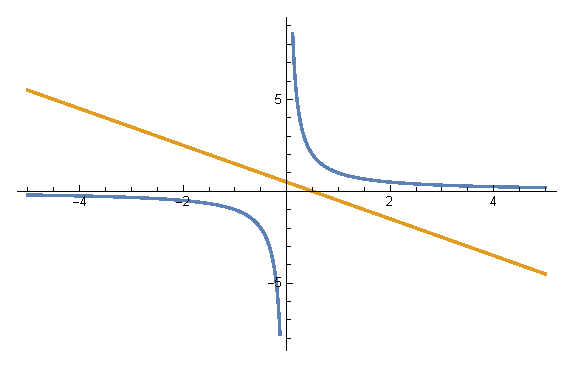
\includegraphics{plots_gr3.eps}
	\caption{Graphs of $x + y = 1/2$ and $xy = 1$}
	\label{fig:plots_gr3}
\end{figure}

and clearly there are no intersections. Moreover, if we have a solution, it will very likely not be unique. This is because if $(x, y)$ solves the system above, so does $(y, x)$ because of the commutativity of addition and multiplication.

How does this even relate to the inverse function theorem? Define $F(x, y) = (x + y, xy)$. Clearly $F$ is $\CD{1}$, with
\[DF(x_0, y_0) = \begin{bmatrix} 1 & 1 \\ y_0 & x_0\end{bmatrix}.\] Then $DF(x_0, y_0)$ is invertible if and only if $x_0 - y_0 \neq 0$. This sort of matches our remarks from earlier: since when $x = y$ we can see that near the intersection point we have local non-invertibility of the function $F$ in question.

Now suppose $x_0 \neq y_0$. Then the inverse function theorem tells us that in some neighborhood $V$ of $(x_0, y_0)$ there exists a bijective mapping $f|V$. So locally there is a solution for $f(x_0, y_0)$. But this doesn't answer our original question: what exactly can $z$ and $w$ be?

Fortunately, or not, we can kill this with elementary observations. The quadratic equation $x^2 -zx + w$ has roots $x$ and $y$. So $x$ and $y$ are real only if 
\[\sqrt{w^2 - 4z} \geq 0 \implies z \leq \frac{w^2}{4}.\]




\section{Differential Forms, the theorems of Vector Calculus}
\subsection{Smooth Paths}
The following section details some brief remarks on paths, their length, and parametrization.

\begin{definition}
A $\mathcal{C}^1$ path in $\Real^n$ is a continuously differentiable function $\gamma: [a, b] \to \Real^n$. $\gamma$ is said to be \textit{smooth} if $\gamma'(t) \neq \mathbf{0}$ for all $t \in [a, b]$.
\end{definition}

The condition $\gamma'(t) \neq \mathbf{0}$ indicates that the direction of a $\mathcal{C}^1$ path cannot change abruptly.

Given a path in $\Real^n$ a natural question one might ask is what is the ``length'' of the path, or how we might define such a concept. Since our path is differentiable there will be some nice theorems about the path length in terms of parametrization of the path. This might be defined here eventually.

Here is the first theorem about path length in terms of the path $\gamma$.
\begin{theorem}
If $\gamma: [a, b] \to \mathbb{R}^n$ is a $\mathcal{C}^1$ path, then the path length $s(\gamma)$ exists, and 
\[s(\gamma) = \int_a^b\norm{\gamma'(t)}~dt.\]
\end{theorem}

If we think of our path $\gamma$ as a moving particle in $\mathbb{R}^n$, whose position vector at time $t$ is $\gamma(t)$, then $\norm{\gamma'(t)}$ is the speed of the particle at time $t$. So the above formula asserts that the distance traveled by the particle is equal to the integral over time of the speed of the particle, which is familiar from elementary calculus.

The actual proof of the theorem is very involved and I will not include it here for now.

Now we introduce the notion of two paths being equivalent. The geometric idea for equivalent paths is as follows. Two $\mathcal{C}^1$ paths are geometrically equivalent if they have the same initial point, the same terminal point, and they trace through the intermediate points in the same order. We also want to ask about whether or not $\alpha$ and $\beta$ have the same length. We will make this equivalence precise now.
\begin{definition}
The path $\alpha: [a, b] \to \Real^n$ is equivalent to $\beta: [c, d] \to \Real^n$ if there is a $\mathcal{C}^1$ function $\varphi: [a, b] \to [c, d]$ such that $\phi([a, b]) = [c, d]$, $\alpha = \beta \circ \varphi$, and $\varphi'(t) > 0$ for all $t$. 
\end{definition}

This relation is actually an equivalence relation. Also, we have that if the $\mathcal{C}^1$ paths $\alpha$ and $\beta$ are equivalent, then $\alpha$ is smooth if and only if $\beta$ is smooth.

The following theorem will show that if $\alpha$ and $\beta$ are equivalent, then their path lengths are equal. (This is the special case $f(x) = 1$.)
\begin{theorem}
Suppose that $\alpha: [a, b] \to \Real^n$ and $\beta: [c, d] \to \Real^n$ are equivalent $\mathcal{C}^1$ paths, and that $f$ is a continuous real-valued function whose domain in $\Real^n$ contains the common image of $\alpha$ and $\beta$. Then we have 
\[\int_a^bf(\alpha(t))\norm{\alpha'(t)}~dt = \int_c^df(\beta(t))\norm{\beta'(t)}~dt.\]
\end{theorem}

\begin{proof}
This will basically be a matter of $u$-substitution. Let $\varphi: [a, b] \to [c, d]$ be a $\mathcal{C}^1$ function such that $\alpha = \beta \circ \varphi$ and $\varphi'(t) > 0$ for all $t \in [a, b]$. Then
\begin{align*}
\int_a^bf(\alpha(t))\norm{\alpha'(t)}~dt &= \int_a^b f(\beta(\varphi(t)))\norm{\beta'(\varphi(t))\varphi'(t)}~dt \\
		&= \int_a^b f(\beta(\varphi(t))) \norm{\beta'(\varphi(t))} \phi'(t)~dt \\
		&= \int_c^d f(\beta(u))\norm{\beta'(u)}~du.
\end{align*}
\end{proof}




\subsection{Line Integrals}
Now that we have considered normal paths, we will consider the idea of a particle travelling and doing work under say a force field. Let $\gamma: [a,b] \to \Real^n$ be a smooth path. We'll think of $\gamma$ as the position vector of a particle moving in $\Real^n$, which is under the influence of a force field $F: \Real^n \to \Real^n$. This means that $F(\gamma(t))$ is the force acting on the particle at time $t$.

If $F$ were a constant force field, then the work done by $F$ moving the particle along a straight line from $\gamma(t_{i-1})$ to $\gamma(t_i)$ by definition would be $F \cdot (\gamma(t_i) - \gamma(t_{i-1})$ (force times displacement).

So just like a path length integral approximation, the sum
\[W(\gamma, F, P) = \sum_{i = 1}^kF(\gamma(t_i)) \cdot (\gamma(t_i) - \gamma(t_{i-1}))\]
as an approximation to the work $W$. Based on the Riemann sum (which converges as expected), we can define the work done by the force field $F$ in moving a particle along $\gamma$ by
\[W = \int_a^b F(\gamma(t)) \cdot \gamma'(t)~dt.\]
In terms of the unit tangent vector
\[T(t) = \frac{\gamma'(t)}{\norm{\gamma'(t)}},\]
we obtain the formula
\[W = \int_a^b F(\gamma(t)) \cdot T(t) \norm{\gamma'(t)}~dt\]
which has the attractive form
\[W = \int_{\gamma}F \cdot T~ds.\]
This says that the work done by the force field is the integral with respect to the pathlength of the ``tangential component'' $F \cdot T$.

In terms of the individual components in $\Real^n$, we have the formula
\[W = \int_a^b [F_1(\gamma(t))\gamma_1'(t) + \cdots + F_n(\gamma(t))\gamma_n'(t)]~dt,\]
or in Leibnizian notation
\[W = \int_a^b \left(F_1\frac{dx_1}{dt} + \cdots + F_n\frac{dx_n}{dt}\right)~dt.\]
Classically we can write this last formula as
\[W = \int_{\gamma}F_1dx_1 + \cdots + F_ndx_n.\]
This type of integral is called a \textbf{line integral} and of course can be defined without any motivation about work done by a particle. 

\begin{definition}
Given a $\mathcal{C}^1$ path $\gamma:[a,b] \to \Real^n$ and $n$ continuous functions $f_1, \dots, f_n$ whose domains in $\Real^n$ contain the image of $\gamma$ the line integral $\int_{\gamma}f_1dx_1 + \cdots + f_ndx_n$ is defined by

\[\int_{\gamma}f_1dx_1 + \cdots + f_ndx_n = \int_a^b [f_1(\gamma(t))\gamma_1'(t) + \cdots + f_n(\gamma(t))\gamma_n'(t)]~dt.\]
\end{definition}

\subsection{An brief introduction to differential forms}

\begin{definition}
A linear \textbf{differential form} on the set $U \subset \Real^n$ is a mapping $\omega$ which associates with each point $x \in U$ a linear function $\omega(x): \Real^n \to \Real$. It is convenient and possibly less confusing to write $\omega(x) = \omega_x$.
\end{definition}

Every linear function $L: \Real^n \to Real$ has the form
\[L(v_1, \dots, v_n) = a_1v_1 + \cdots + a_nv_n = a_1p_1(v) + \cdots + a_np_n(v)\]
where $p_i$ denotes the projection function of $v$ onto the $i$th component. Then if we use the notation $p_i = dx_i$ then the above formula becomes
\[L = a_1dx_1 + \cdots + a_ndx_n.\] If $L = \omega(x)$ depends on the point $x$ then so do the coefficients $a_1, \dots, a_n$, giving us the following result.

\begin{proposition}
If $\omega$ is a differential form on $U \subset \Real^n$, then there exist unique real-valued functions $a_1, \dots, a_n$ on $U$ such that 
\[\omega(x) = \omega_x = a_1(x)dx_1 + \cdots + a_n(x)dx_n.\]
$\omega$ is said to be continuous (or differentiable, or $\CD{1}$) if its coefficient functions $a_1, \dots, a_n$ are continous (or differentiable, or $\CD{1}$). 
\end{proposition}

Then for each $x \in U$ this expression just denotes the linear function whose value at $v$ is
\[\omega_x(v) = a_1(x)v_1 + \cdots + a_n(x)v_n.\]

\begin{definition}
Let $\omega$ be a continuous differential form on $U \subset \Real^n$ and $\gamma:[a,b] \to U$ a $\CD{1}$ path. We define the integral of $\omega$ over the path $\gamma$ by 
\[\int_{\gamma}\omega = \int_a^b \omega_{\gamma(t)}(\gamma'(t))~dt.\]
In other words, if $\omega = a_1dx_1 + \cdots + a_ndx_n$, then
\[\int_{\gamma}\omega = \int_a^b[a_1(\gamma(t))\gamma_1'(t) + \cdots + a_n(\gamma(t))\gamma_n'(t)]~dt.\]
\end{definition}

Observe that a line integral is simply the integral of the differential form appearing as its ``integrand''.

\subsection{Examples}

\begin{example}
Let $\omega$ be the differential form defined on $\mathbb{R}^2 - \{0\}$ by 
\[\omega = \frac{-ydx + xdy}{x^2 + y^2}.\]
If $\gamma_1: [0, 1] \to \Real^2 - \{0\}$ is defined by $\gamma_1(t) = (\cos(\pi t), \sin(\pi t))$, the the image of $\gamma_1$ is the upper half of the unit circle. We can calculate
\[\int_{\gamma_1}\omega = \pi.\]
\end{example}

\begin{example}
Let $U$ denote $\Real^2$ minus the nonnegative $x$ axis. Let $\theta: U \to \Real$ be defined by $\theta(x, y) = \arctan(y/x)$.

Then $d\theta$ will be the differential form in the previous example.
\end{example}

The following theorem is a certain generalization of the fundamental theorem of calculus for paths in $\Real^n$.
\begin{theorem}
If $f$ is a real valued $\CD{1}$ function on the open set $U \subset \Real^n$, and $\gamma:[a, b] \to U$ is a $\CD{1}$ path, then 
\[\int_{\gamma}df = f(\gamma(b)) - f(\gamma(a)).\]

In other words, the line integral of the differential will be independent of the path taken, it only depends on the endpoints of the path.
\end{theorem}

\begin{proof}
Essentially we will reduce this to the fundamental theorem of calculus. Define $g: [a, b] \to \Real$ by $g = f \circ \gamma$. Then by the chain rule, $g'(t) = \nabla f(\gamma(t)) \cdot \gamma'(t)$. Then we have that
\begin{align*}
\int_{\gamma}df &= \int_a^b df_{\gamma(t)}(\gamma'(t))~dt \\
		&= \int_a^b [D_1f(\gamma(t))\gamma_1'(t) + \cdots + D_nf(\gamma(t))\gamma_n'(t)]~dt \\
		&= \int_a^b \nabla f(\gamma(t)) \cdot \gamma'(t)~dt \\
		&= \int_a^b g'(t)~dt \\
		&= g(b) - g(a) = f(\gamma(b)) - f(\gamma(a)).
\end{align*}
\end{proof}


\subsection{Green's Theorem}
In this section we will outline Green's Theorem and illustrate a couple of examples.

Recall the fundamental theorem of calculus
\[\int_a^bf'(t)~dt = f(b) - f(a)\]
(where $f$ is $\CD{1}$). We may regard the interval $I = [a, b]$ as an oriented smooth curve from $a$ to $b$, and we might write $\int_Idf$ for the left hand side of the above equation. Thinking of $b$ as the positive endpoint and $a$ as the negative endpoint of $I$, we can write $\int_{\partial I}f$ instead of $f(b) - f(a)$. Then the FTC takes on sort of a contrived form
\[\int_Idf = \int_{\partial I}f.\]

What is Green's Theorem? Well, it's a certain generalization of the fundamental theorem of calculus, and we will state it in the form of the modified equation above.

\begin{definition}
Given a $\CD{1}$ differential form $\omega = Pdx + Qdy$ in two variables, the differential $d\omega$ is defined by 
\[d\omega = \left(\frac{\partial Q}{\partial x} - \frac{\partial P}{\partial y}\right)~dx~dy.\] We call $d\omega$ a \textit{differential $2$-form}.
\end{definition}

\begin{definition}
Given a continuous differential $2$-form $\alpha = adxdy$ and a contented set $D \subset \Real^2$, the integral of $\alpha$ on $D$ is defined by 
\[\int_D\alpha = \iint_D a(x, y)~dx~dy.\]
\end{definition}

Now we are ready for the statement of Green's Theorem, as stated below.

\begin{theorem}
Let $D \in \Real^2$ be a connected compact set whose boundary $\partial D$ is the union of a finite number of mutually disjoint piecewise-smooth closed curves. Suppose each of these curves is positively oriented (interior is on the left hand side) with respect to $D$. If $\omega = Pdx + Qdy$ is a $\CD{1}$ differential $1$-form defined on $D$, then 
\[\int_Dd\omega = \int_{\partial D}\omega.\]
More explicitly, we have that
\[\iint_D\left(\frac{\partial Q}{\partial x} - \frac{\partial P}{\partial y}\right)~dx~dy = \int_{\partial D}Pdx + Qdy.\]
\end{theorem}


\end{document}
